
\chapter{GCSE Revision: Functions and Function Transformation Questions}

\begin{enumerate}
  \item \mrk{3}
  \begin{figure}[H]
    \centering
    \textbf{A}
    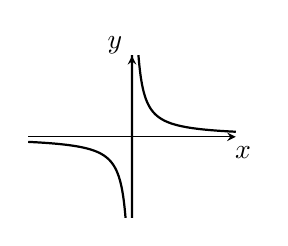
\begin{tikzpicture}
      \begin{axis}[
          xmin = -8, xmax = 8,
          ymin = -8, ymax = 8,
          xticklabels = {},
          yticklabels = {},
          xtick = {0},
          ytick = {0},
          axis lines = middle,
          height = 0.3\textwidth,
          x label style={at={(ticklabel* cs:0.95)},anchor=north west},
          y label style={at={(ticklabel* cs:0.95)},anchor=south east},
          xlabel = {$x$},
          ylabel = {$y$},
        ]
        % Plot a function
        \addplot[
          domain = -8:8,
          samples = 200,
          smooth,
          thick,
        ] {4/x};
      \end{axis}
    \end{tikzpicture}
    \hspace*{1cm}
    \textbf{B}
    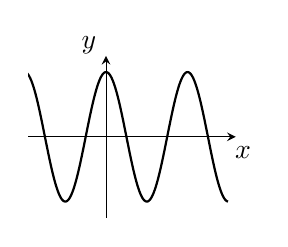
\begin{tikzpicture}
      \begin{axis}[
          xmin = -6, xmax = 10,
          ymin = -5, ymax = 5,
          xticklabels = {},
          yticklabels = {},
          xtick = {0},
          ytick = {0},
          axis lines = middle,
          height = 0.3\textwidth,
          x label style={at={(ticklabel* cs:0.95)},anchor=north west},
          y label style={at={(ticklabel* cs:0.95)},anchor=south east},
          xlabel = {$x$},
          ylabel = {$y$},
        ]
        % Plot a function
        \addplot[
          domain = -6.4:9.4,
          samples = 200,
          smooth,
          thick,
        ] {4*cos(deg(x))};
      \end{axis}
    \end{tikzpicture}\par
    \textbf{C}
    \begin{tikzpicture}
      \begin{axis}[
          xmin = -2, xmax = 1.5,
          ymin = -2, ymax = 6,
          xticklabels = {},
          yticklabels = {},
          xtick = {0},
          ytick = {0},
          axis lines = middle,
          height = 0.3\textwidth,
          x label style={at={(ticklabel* cs:0.95)},anchor=north west},
          y label style={at={(ticklabel* cs:0.95)},anchor=south east},
          xlabel = {$x$},
          ylabel = {$y$},
        ]
        % Plot a function
        \addplot[
          domain = -2:1,
          samples = 200,
          smooth,
          thick,
        ] {4*2^x};
      \end{axis}
    \end{tikzpicture}
    \hspace*{1cm}
    \textbf{D}
    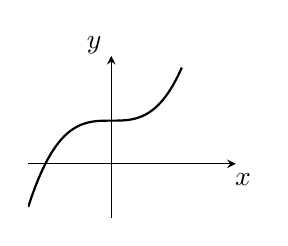
\begin{tikzpicture}
      \begin{axis}[
          xmin = -2, xmax = 3,
          ymin = -5, ymax = 10,
          xticklabels = {},
          yticklabels = {},
          xtick = {0},
          ytick = {0},
          axis lines = middle,
          height = 0.3\textwidth,
          x label style={at={(ticklabel* cs:0.95)},anchor=north west},
          y label style={at={(ticklabel* cs:0.95)},anchor=south east},
          xlabel = {$x$},
          ylabel = {$y$},
        ]
        % Plot a function
        \addplot[
          domain = -2:1.7,
          samples = 200,
          smooth,
          thick,
        ] {x^3+4};
      \end{axis}
    \end{tikzpicture}\par
    \textbf{E}
    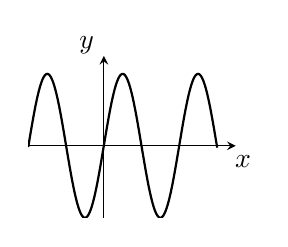
\begin{tikzpicture}
      \begin{axis}[
          xmin = -6.3, xmax = 11,
          ymin = -4, ymax = 5,
          xticklabels = {},
          yticklabels = {},
          xtick = {0},
          ytick = {0},
          axis lines = middle,
          height = 0.3\textwidth,
          x label style={at={(ticklabel* cs:0.95)},anchor=north west},
          y label style={at={(ticklabel* cs:0.95)},anchor=south east},
          xlabel = {$x$},
          ylabel = {$y$},
        ]
        % Plot a function
        \addplot[
          domain = -6.3:9.45,
          samples = 200,
          smooth,
          thick,
        ] {4*sin(deg(x))};
      \end{axis}
    \end{tikzpicture}
    \hspace*{1cm}
    \textbf{F}
    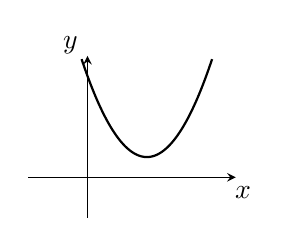
\begin{tikzpicture}
      \begin{axis}[
          xmin = -2, xmax = 5,
          ymin = -2, ymax = 6,
          xticklabels = {},
          yticklabels = {},
          xtick = {0},
          ytick = {0},
          axis lines = middle,
          height = 0.3\textwidth,
          x label style={at={(ticklabel* cs:0.95)},anchor=north west},
          y label style={at={(ticklabel* cs:0.95)},anchor=south east},
          xlabel = {$x$},
          ylabel = {$y$},
        ]
        % Plot a function
        \addplot[
          domain = -0.2:4.2,
          samples = 200,
          smooth,
          thick,
        ] {x^2-4*x+5};
      \end{axis}
    \end{tikzpicture}
  \end{figure}
  Each equation in the table represents one of the graphs \textbf{A} to \textbf{F}.\\
  Write the letter of each graph in the correct place in the table.
  \begin{table}[H]
    \centering
    \begin{tabular}{| l | l |} 
      \hline
      \textbf{Equation} & \textbf{Graph} \\
      \hline
      $y = 4\sin x^\circ$ &  \\ 
      \hline
      $y = 4\cos x^\circ$ &  \\
      \hline
      $y = x^2 - 4x + 5$ & \\
      \hline
      $y = 4 \times 2^x$ & \\
      \hline
      $y = x^3 + 4$ & \\
      \hline
    \end{tabular}
  \end{table}
  \item \mbox{}
  \begin{enumerate}
    \begin{figure}[H]
      \centering
      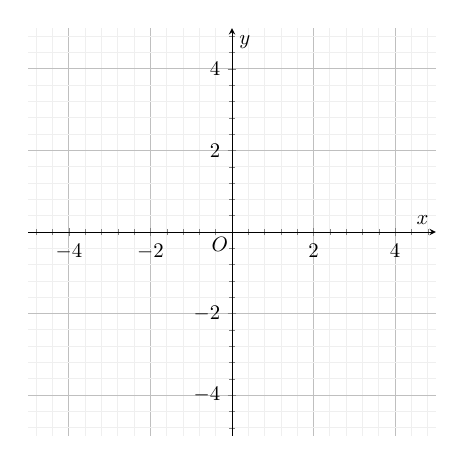
\begin{tikzpicture}[scale=0.75]
        \begin{axis}[
            xmin = -5, xmax = 5,
            ymin = -5, ymax = 5,
            grid = both,
            minor tick num = 4,
            major grid style = {lightgray},
            minor grid style = {lightgray!25},
            axis lines = middle,
            width = 0.7\textwidth,
            height = 0.7\textwidth,
            xlabel = {$x$},
            ylabel = {$y$},
          ]
          \node at (-0.3, -0.3) {$O$};
        \end{axis}
      \end{tikzpicture}
    \end{figure}
    \item On the grid, draw the graph of $x^2 + y^2 = 4$.\mrk{2}
    \begin{figure}[H]
      \centering
      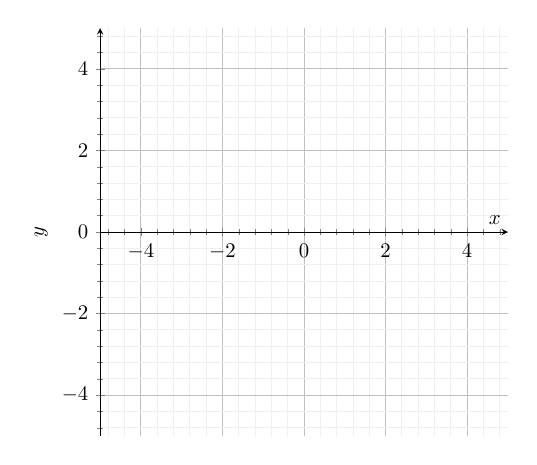
\begin{tikzpicture}[scale=0.75]
        \begin{axis}[
            xmin = -5, xmax = 5,
            ymin = -5, ymax = 5,
            grid = both,
            minor tick num = 4,
            major grid style = {lightgray},
            minor grid style = {lightgray!25},
            axis y line = left, 
            axis x line = middle,
            width = 0.7\textwidth,
            height = 0.7\textwidth,
            xlabel = {$x$},
            ylabel = {$y$},
          ]
          \end{axis}
        \end{tikzpicture}
      \end{figure}
      \item On the grid, sketch the graph of $y = \cos x$ for $\ang{0} \leq x \leq \ang{360}$.\mrk{2}
  \end{enumerate}
  \item %
  \begin{enumerate}
    \item Complete the table of values for $y = x^3 - 7$.\mrk{2}
    \begin{table}[H]
      \centering
      \begin{tabular}{|m{1cm}|m{1cm}|m{1cm}|m{1cm}|m{1cm}|m{1cm}|m{1cm}|} 
        \hline
        $x$ &	-2 & -1 &	0 &	1 &	2 &	3 \\
        \hline
        $y$ & -8 & & & & & 20 \\
        \hline
      \end{tabular}
    \end{table}
    \item On the grid, draw the graph of $y = x^3 - 7$ for values of $x$ from $-2$ to $3$.\mrk{2}
    \begin{figure}[H]
      \centering
      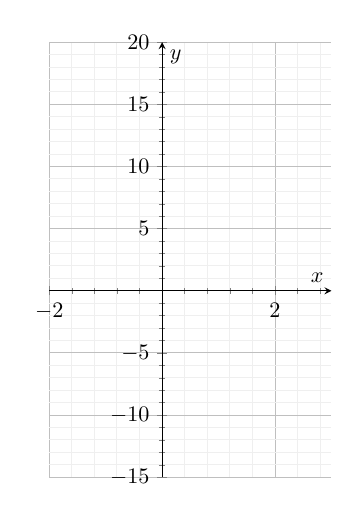
\begin{tikzpicture}[scale=0.8]
        \begin{axis}[
            xmin = -2, xmax = 3,
            ymin = -15, ymax = 20,
            grid = both,
            minor tick num = 4,
            major grid style = {lightgray},
            minor grid style = {lightgray!25},
            axis lines = middle,
            width = 0.5\textwidth,
            height = 0.7\textwidth,
            xlabel = {$x$},
            ylabel = {$y$},
          ]
          \end{axis}
        \end{tikzpicture}
      \end{figure}
  \end{enumerate}
  \item %
  \begin{enumerate}
    \item Construct the graph of $x^2 + y^2 = 9$.
    \begin{figure}[H]
      \centering
      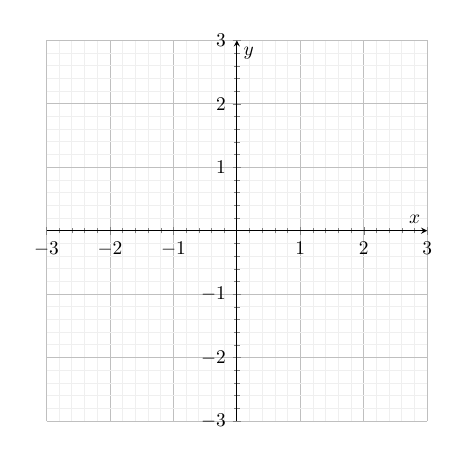
\begin{tikzpicture}[scale=0.7]
        \begin{axis}[
            xmin = -3, xmax = 3,
            ymin = -3, ymax = 3,
            grid = both,
            minor tick num = 4,
            major grid style = {lightgray},
            minor grid style = {lightgray!25},
            axis lines = middle,
            width = 0.7\textwidth,
            height = 0.7\textwidth,
            xlabel = {$x$},
            ylabel = {$y$},
          ]
          \end{axis}
        \end{tikzpicture}
      \end{figure}
      \item By drawing the line $x + y = 1$ on the grid, solve the equations
      \begin{align*}
        x^2 + y^2 &= 9\\
        x + y &= 1
      \end{align*}
  \end{enumerate}
  \item %
  \begin{enumerate}
    \item Complete the table of values for $y = x^2 + x - 3$.\mrk{2}
    \begin{table}[H]
      \centering
      \begin{tabular}{|m{1cm}|m{1cm}|m{1cm}|m{1cm}|m{1cm}|m{1cm}|m{1cm}|m{1cm}|} 
        \hline
        $x$	& -4 & -3 & -2 & -1 &	0 &	1 &	2 \\
        \hline
        $y$ & 9 & & -1 & -3 & & & 3 \\
        \hline
      \end{tabular}
    \end{table}
    \item On the grid below, draw the graph of $y = x^2 + x - 3$ for values of $x$ from $-4$ to $2$.\mrk{2}
    \begin{figure}[H]
      \centering
      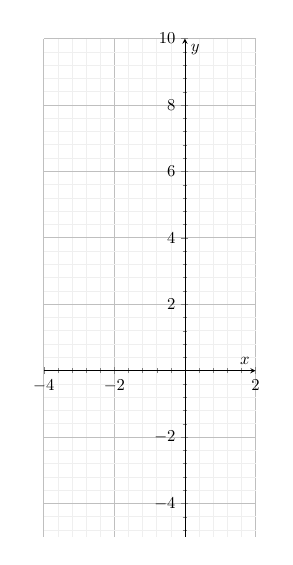
\begin{tikzpicture}[scale=0.6]
        \begin{axis}[
            xmin = -4, xmax = 2,
            ymin = -5, ymax = 10,
            grid = both,
            minor tick num = 4,
            major grid style = {lightgray},
            minor grid style = {lightgray!25},
            axis lines = middle,
            width = 0.5\textwidth,
            height = \textwidth,
            xlabel = {$x$},
            ylabel = {$y$},
          ]
          \end{axis}
        \end{tikzpicture}
      \end{figure}
  \end{enumerate}
  \item The graph of $y = f(x)$ is shown on each of the grids.
  \begin{enumerate}
    \item On this grid, sketch the graph of $y = f(x - 3)$.\mrk{2}
    \begin{figure}[H]
      \centering
      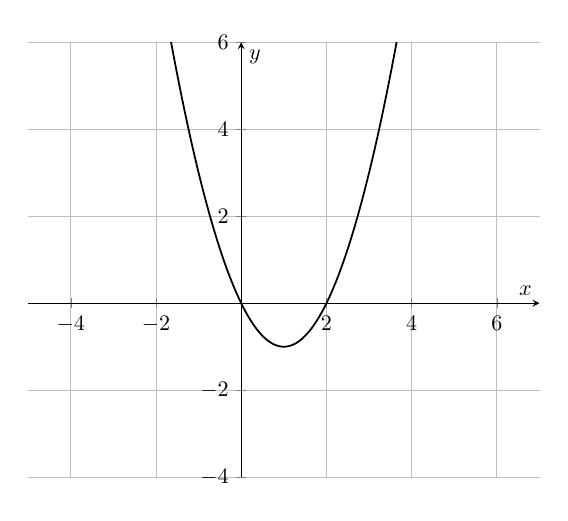
\begin{tikzpicture}[scale=0.8]
        \begin{axis}[
            xmin = -5, xmax = 7,
            ymin = -4, ymax = 6,
            grid = both,
            axis lines = middle,
            width = 0.8\textwidth,
            height = 0.7\textwidth,
            xlabel = {$x$},
            ylabel = {$y$},
          ]
          % Plot a function
          \addplot[
            domain = -2:4,
            samples = 200,
            smooth,
            thick,
          ] {x^2 - 2*x};
          \end{axis}
        \end{tikzpicture}
      \end{figure}
      \item On this grid, sketch the graph of $y = 2f(x)$.\mrk{2}
      \begin{figure}[H]
        \centering
        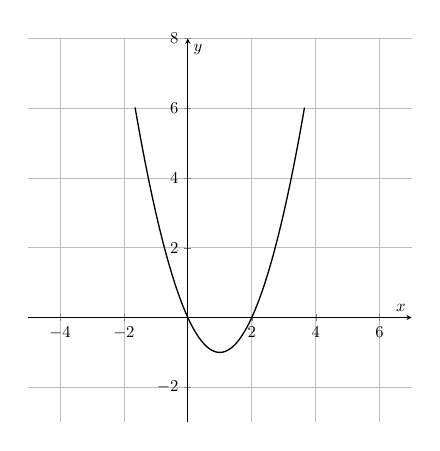
\begin{tikzpicture}[scale=0.6]
          \begin{axis}[
              xmin = -5, xmax = 7,
              ymin = -3, ymax = 8,
              grid = both,
              axis lines = middle,
              width = 0.8\textwidth,
              height = 0.8\textwidth,
              xlabel = {$x$},
              ylabel = {$y$},
            ]
            % Plot a function
            \addplot[
              domain = -1.65:3.65,
              samples = 200,
              smooth,
              thick,
            ] {x^2 - 2*x};
            \end{axis}
          \end{tikzpicture}
        \end{figure}
  \end{enumerate}
  \item The graph of $y = f(x)$ is shown on the grids.
  \begin{enumerate}
    \item On this grid, sketch the graph of $y = f(x - 3)$.\mrk{2}
  \end{enumerate}
  

\end{enumerate}